% LaTeX template for Lab Reports
% Copyright (C) 2014 Julian Coy

%% CHANGE REPORT TITLE HERE
\newcommand{\reporttitle}{
 FSM System Design
}

%% HEADER/PREAMBLE INFORMATION

% "The font should be 11pt Times New Roman"
\documentclass[11pt]{report}
\usepackage[T1]{fontenc}
\usepackage[utf8]{inputenc}

\usepackage{mathptmx}               

% "The body of the paper should use 1" margins on all sides."
\usepackage[margin=1in]{geometry}

% "Pages must be numbered, starting with 1 on the first page in the body of the report.
% The cover page should not be numbered. 
% Page numbers should be in the bottom-right corner of the page."
\usepackage{fancyhdr}
\pagestyle{fancy}
\fancyhead{}
\fancyfoot{}
\renewcommand{\headrulewidth}{0pt}
\fancyfoot[R]{\thepage}

% Set up customized spacing
\usepackage{setspace}

% Allows for Trademark Symbols
\usepackage{textcomp}

% Remove spacing between items in lists
\usepackage{enumitem}

% Remove extra spacing between titles of sections and subsections
\usepackage{titlesec}
\titlespacing\section{0pt}{10pt}{10pt}
\titlespacing\subsection{0pt}{10pt}{10pt}
\titlespacing\subsubsection{0pt}{0pt plus 4pt minus 2pt}{0pt plus 2pt minus 2pt}

% Setup the specialized chapter section for the Abstract
\titlespacing\chapter{0pt}{0pt plus 4pt minus 2pt}{0pt plus 2pt minus 2pt}
\titleformat{\chapter}[block]{\centering\Huge}{}{}{}{}

% Set up BibTeX integration using IEEE citation format
\usepackage{cite}
\bibliographystyle{ieeetr}
\usepackage{url}

% Set bibliography to have a section header rather than chapter header
\makeatletter
\renewenvironment{thebibliography}[1]
     {\section*{\scshape Works Cited}% <-- this line was changed from \chapter* to \section*
      \@mkboth{\MakeUppercase\bibname}{\MakeUppercase\bibname}%
      \list{\@biblabel{\@arabic\c@enumiv}}%
           {\settowidth\labelwidth{\@biblabel{#1}}%
            \leftmargin\labelwidth
            \advance\leftmargin\labelsep
            \@openbib@code
            \usecounter{enumiv}%
            \let\p@enumiv\@empty
            \renewcommand\theenumiv{\@arabic\c@enumiv}}%
      \sloppy
      \clubpenalty4000
      \@clubpenalty \clubpenalty
      \widowpenalty4000%
      \sfcode`\.\@m}
     {\def\@noitemerr
       {\@latex@warning{Empty `thebibliography' environment}}%
      \endlist}
\makeatother

% Set up math
\usepackage{amsmath}
\usepackage{amsfonts}
\usepackage{amssymb}

% Set up graphics
\usepackage{graphicx}
\usepackage{float}

% Set up tables
\usepackage{tabularx}
\usepackage{booktabs}

% Set up code blocks
% or not...

\usepackage{listings}
\usepackage{color}

\definecolor{dkgreen}{rgb}{0,0.6,0}
\definecolor{gray}{rgb}{0.5,0.5,0.5}
\definecolor{mauve}{rgb}{0.58,0,0.82}

\lstset{frame=tb,
  language=VHDL,
  aboveskip=3mm,
  belowskip=3mm,
  showstringspaces=false,
  columns=flexible,
  basicstyle={\small\ttfamily},
  numbers=none,
  numberstyle=\tiny\color{gray},
  keywordstyle=\color{blue},
  commentstyle=\color{dkgreen},
  stringstyle=\color{mauve},
  breaklines=true,
  breakatwhitespace=true
  tabsize=3
}

%% START OF DOCUMENT

\begin{document}

% "The main body of text should use 1.5 spacing"
\begin{spacing}{1.5}

% Suppress page numbering on first page
\thispagestyle{empty}

\begin{scshape}

% Title
% "The title should be centered and written in approximately 22pt font."
\vspace*{30pt}
{
\Huge
\begin{center}
    \reporttitle
\end{center}
}
\vspace{30pt}

% Team Number
% "The Team number should be centered and written several lines below the title and should use a
% similar size font as the title."
{
\Large
\begin{center}
  Lab Report 2 for ECE327 \\
  Digital Systems Design
\end{center}
}
\vspace{30pt}
% Team Members
% "Directly below the team identifier, team members should be listed alphabetically by last name, one
% per line, in approximately 14pt font. The column of names should be approximately centered on
% the page, but the names within the column should be left justified (so they all start at the same
% horizontal position)."
{
\Large 
\begin{center}
  Submitted by \\
  Julian Coy
\end{center}
}
\vspace{120pt}

{
\Large
\begin{center}
  Undergraduate of Electrical \& Computer Engineering \\
  Clemson University
\end{center}
}
\vspace{30pt}

{
\Large
\begin{center}
  March 12, 2014
\end{center}
}

\end{scshape}

% New page and reset page numbering
\clearpage

%% START EDITS BELOW %%

\vspace{15pt}
  \setcounter{chapter}{1}
  \chapter*{Abstract}
  \label{cha:abstract}
\vspace{72pt}

Finite state machines (FSMs) are the basic building blocks of complex computing.  They allow for logical implementation of algorithms, which is critical to the engineering of computing systems.  In this lab, a finite state machine is constructed to flag "stop codons" in a sample of DNA code.  The implementation of this FSM is done though VHDL using behavioral modeling techniques.  Testbench results are provided later in this report to show a working simulation of the FSM when connected to other logical components.  The other logical components built for this lab are a Parallel-to-Serial Output (PISO) register and a counter register.  The inputs to the FSM design are threefold.  There is one array of 18 switches which is used to simulate the DNA input.  There is also be a "reset" button and a "load" button.  The reset button asynchronously resets the counter block, while the load button pushes new data into the PISO register. This design showcases the power of finite state machine logic.  It is critical for engineers to grasp the power of logical computation and to see the scalability of such power.  By combining simple FSM logical blocks, one can create a vast and complicated algorithm with ease.

\vspace{3.5in}

\textit{Note: All clocks generated for simulation were built using Morten Zilmers clock gen package \cite{Synth}.}

\thispagestyle{empty} % clear page number
\clearpage
\setcounter{page}{1}

\section*{\scshape Introduction} %(0.5 pages)
\label{cha:introduction}

The purpose of this lab is to sequence DNA bases consisting of "T", "A", "C", and "G" and look for stop codons.  Stop codons are series of three bases that trigger the end of a DNA sequence.  The stop codons we look for in this lab are "TAA", "TGA", and "TAG".  In order to differentiate the bases, we use a binary representation for the bases (Figure \ref{fig:bases}).  The bases are then fed into the FSM, the number of stop codons are counted, and then the count is displayed on the Altera board.

\vspace{15px}
\begin{figure}[H]
    \centering
    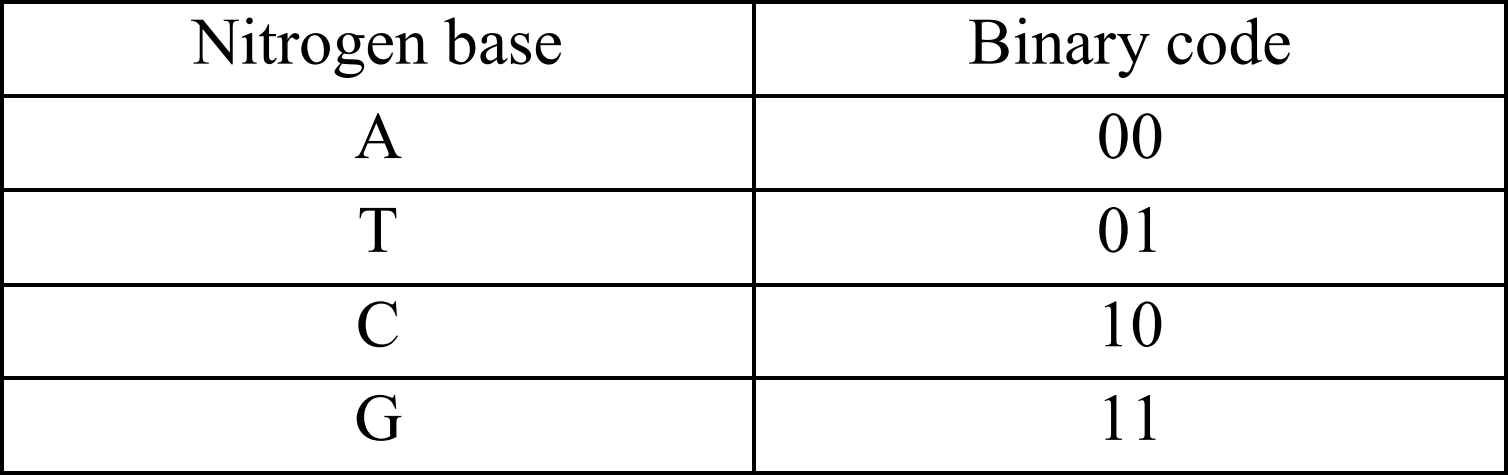
\includegraphics[width=0.6\textwidth,keepaspectratio]{bases.png}
    \caption{DNA Base Representation}
    \label{fig:bases}
\end{figure}

Lab 2 consists of three major logical components: the FSM logic, the counter logic, and the PISO logic. There is also one minor component, the LED logic.  The counter and PISO components are standalone and can be simulated through ModelSim for testing or used for implementation with other systems with minimal modifications.  The FSM logic is designed to model state transitions of the incoming DNA data from the PISO.  The minor LED logic simply displays a number of LEDs correspondent to the output of the counter logic.

\section{\scshape Lab 2 System Design} %(0.5 pages)
\label{sec:fsm_design}

\subsection{\scshape PISO Logic Design}
\label{sub:design_piso}

The PISO component for this lab was built specifically to handle 18 bits of input data at a time.  This was a design choice made for the layout of the Altera board, as it only allowed for 18 bits of modifiable input at a time. The PISO logic parses the 18 bits of data by 2 bit intervals.  It then outputs the first two bits of data on the rising edge of the clock.  This output is connected to the FSM input.  The PISO then shifts the data left by two bits and adds a "01" to the right end.  The "01" code was chosen for the shift packing to make sure that when the data is fully read, no extra stop codons are accidentally detected.  Since the code for the "T" base is "01" and no stop codons end with "T" or consist of all "T" bases, this eliminates that possibility.

\subsection{\scshape Testing of the PISO}
\label{sub:test_piso}

To test the PISO, a testbench was created that would send in a string of data to the PISO and monitor the output on the rising edge of the following clock cycles (Figure \ref{fig:test_piso}). Notice that the output data is not started until the rising edge of the clock cycle following the release of the load button (low active).  In the example shown, the data input is "01001100010101001" which corresponds to "TAGATTTAT".  The output is exactly what we expect. Not shown in the figure is the loading of "T" ("01") values on the preceeding end because it shows no change to the final value in the simulation.

\vspace{15px}
\begin{figure}[H]
    \centering
    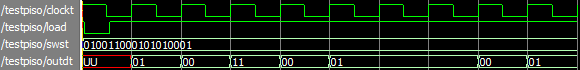
\includegraphics[width=1.0\textwidth,keepaspectratio]{piso.png}
    \caption{PISO Simulation Results}
    \label{fig:test_piso}
\end{figure}

\subsection{\scshape Counter Logic Design}
\label{sub:design_counter}

The counter is modeled behaviorally and simply counts the number of stop flags from the FSM it encounters.  The maximum count used for this project is three, but can be modified to much larger ranges with only a few lines of code.  The counter outputs its value on an integer signal that is sent to the LED logic.

\subsection{\scshape Testing of the Counter}
\label{sub:test_counter}

The counter was tested by sending stop flags to the input and periodically sending a reset signal (Figure \ref{fig:test_counter}).  The counter performed without issue even when using large integer values.  The maximum count size tested was 255, but since the maximum number of stop codons possible from the board were three, the counter integer limit was set to 3.

\vspace{15px}
\begin{figure}[H]
    \centering
    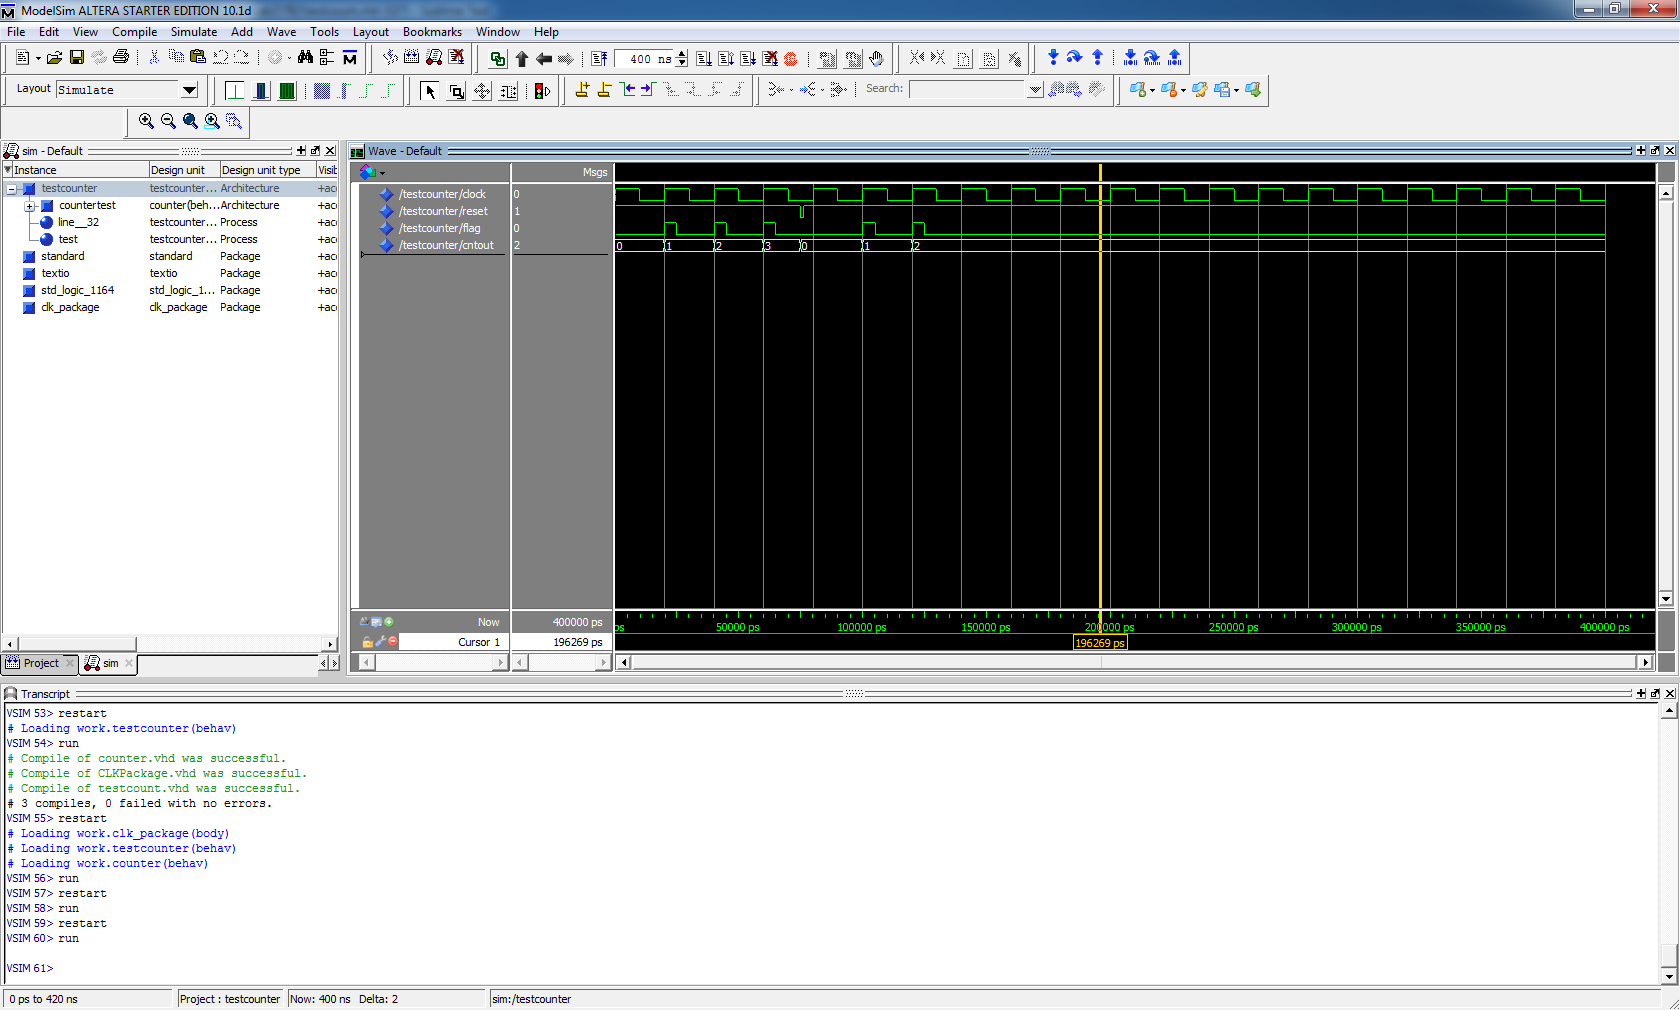
\includegraphics[width=0.8\textwidth,height=4cm,keepaspectratio]{counter.png}
    \caption{Counter Simulation Results\cite{Synth}}
    \label{fig:test_counter}
\end{figure}

\subsection{\scshape FSM Logic Design}
\label{sub:design_counter}

The FSM was designed with 4 logical states: A, B, C, and D.  The first state, A, was the reset state.  This state represents no stop codons and no detection of the beginning of any codons (which always start with a "T" base).  Once a "T" is detected the state will shift to B.  From B there are four options which are shown in Figure \ref{fig:diag_fsm}.  In the figure, the input to the FSM "w" determines the next state.  This FSM uses a Mealy design principle.  This allows for faster outputs and less state management.  In fact, to implement this in a Moore model, at least 5 states would need to be used.

\vspace{15px}
\begin{figure}[H]
    \centering
    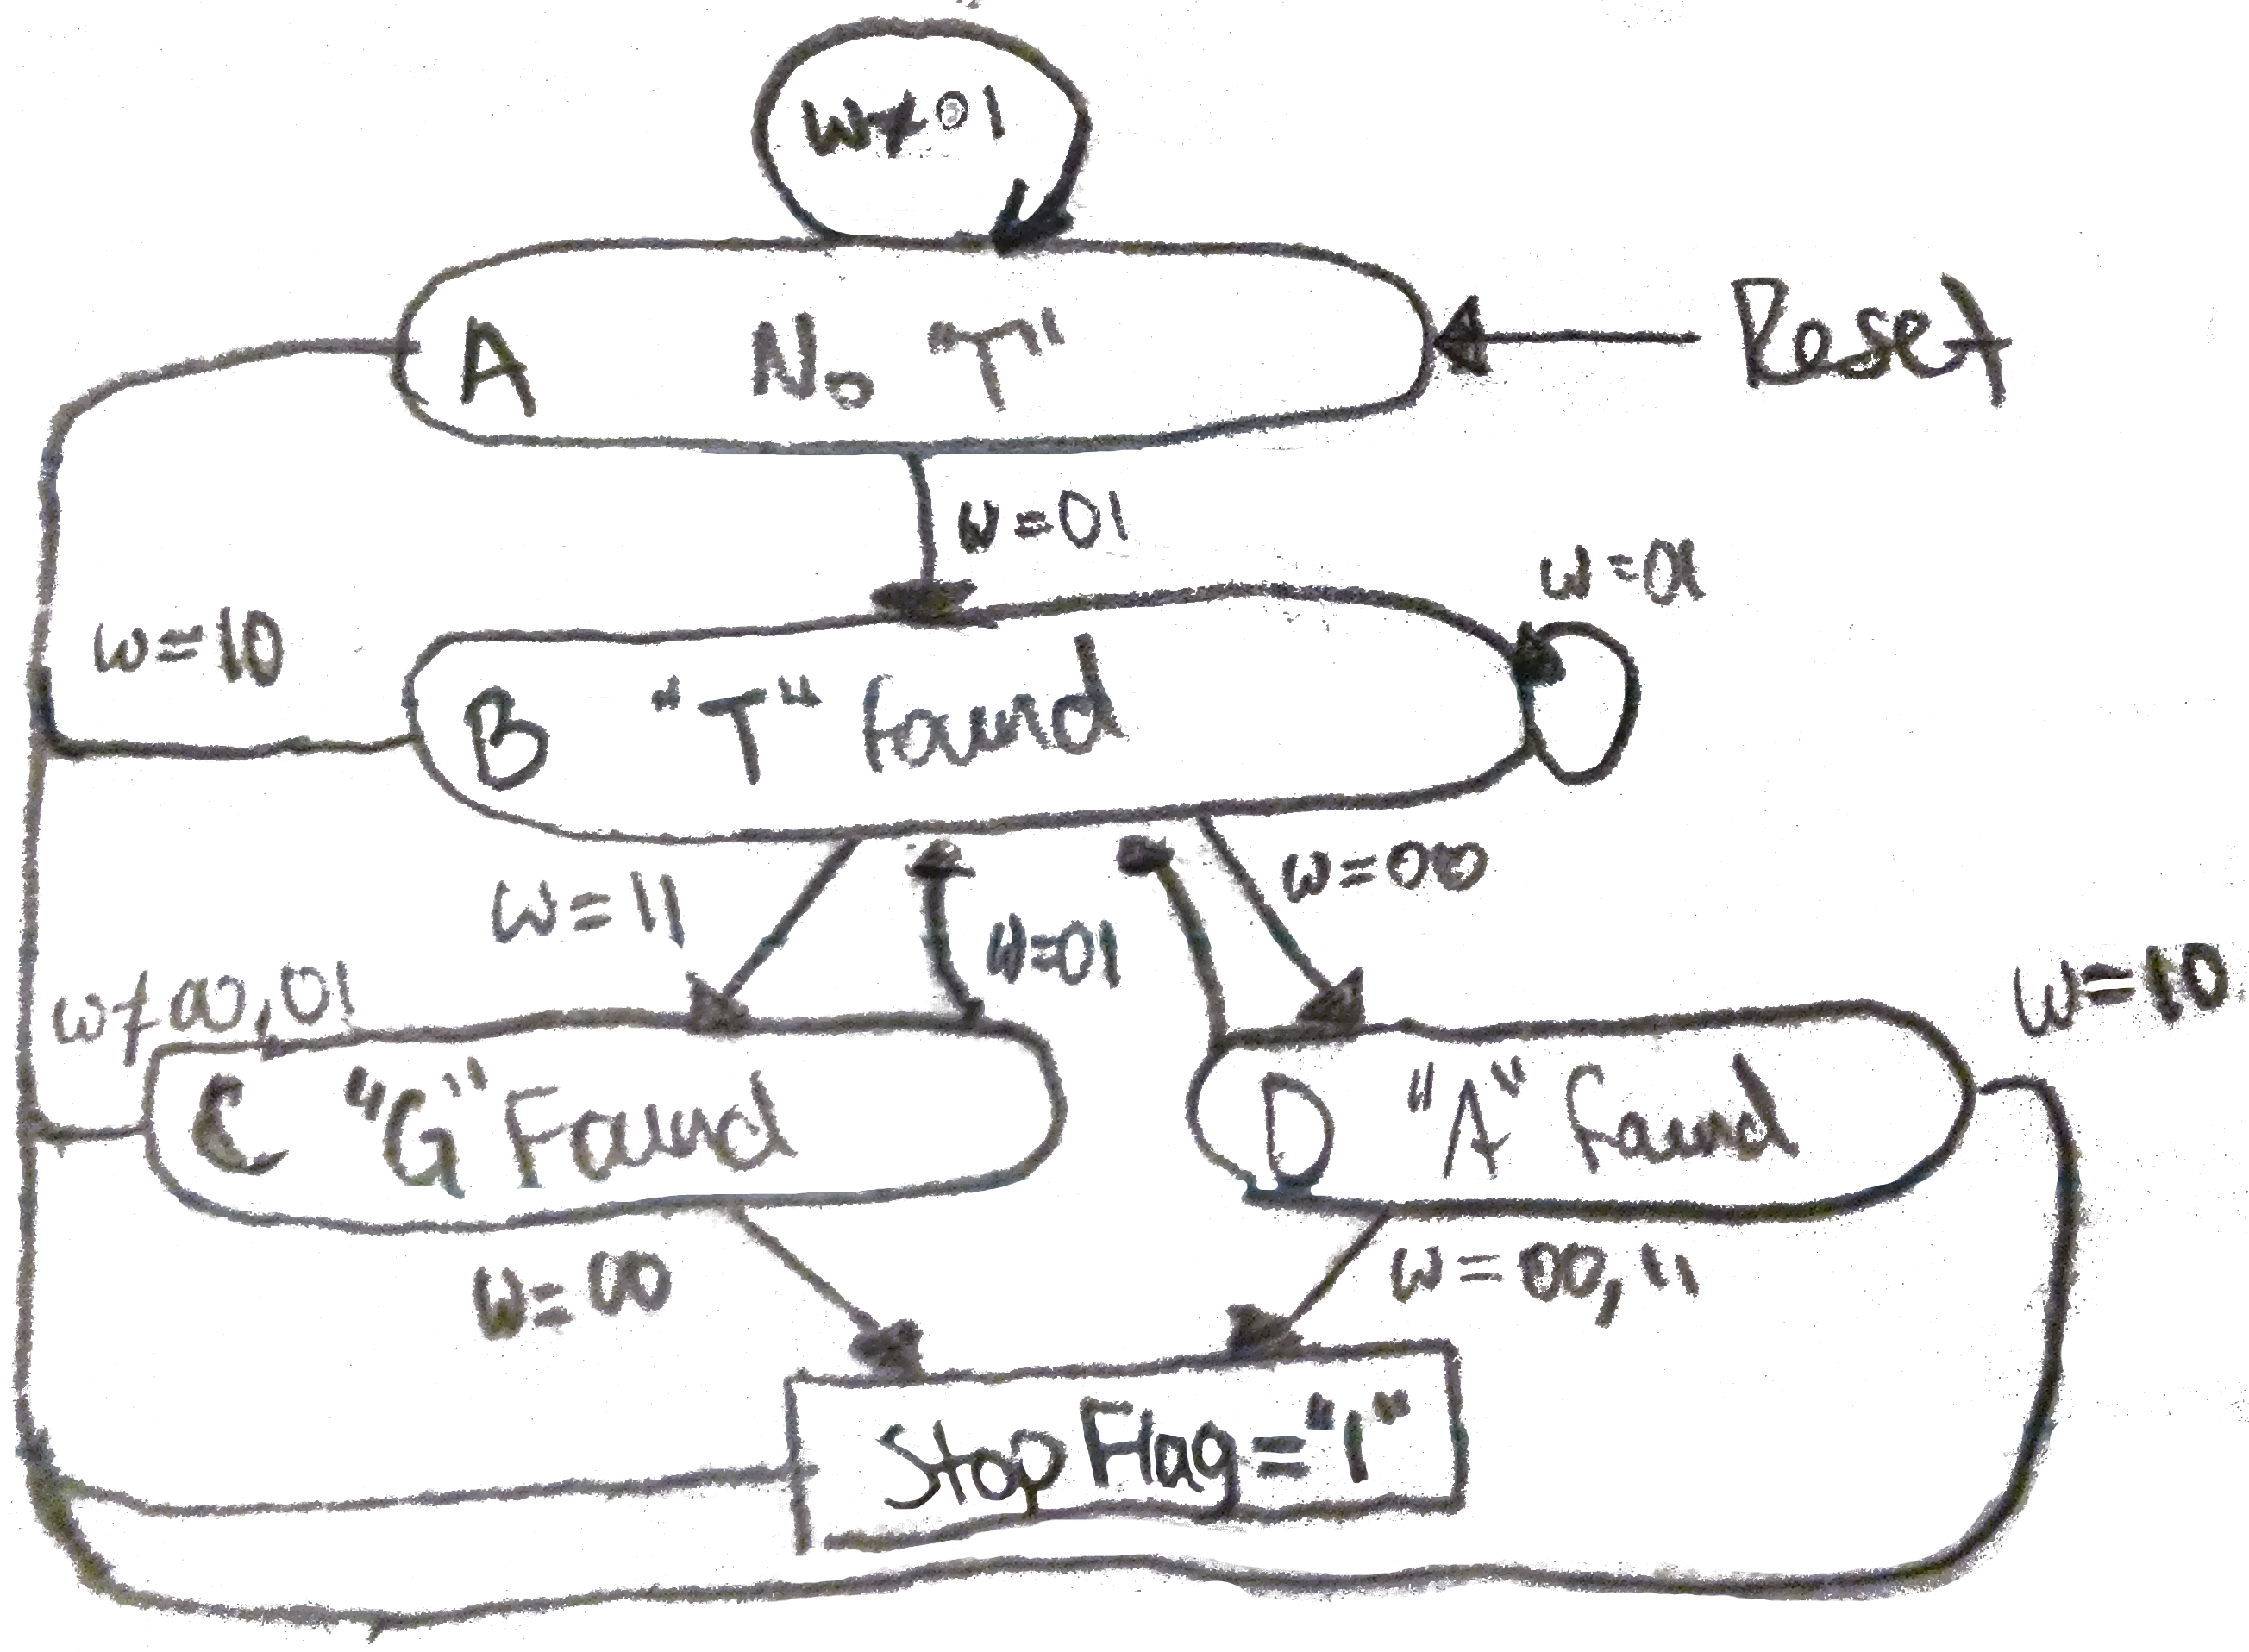
\includegraphics[width=0.7\textwidth,keepaspectratio]{fsm.png}
    \caption{FSM State Diagram}
    \label{fig:diag_fsm}
\end{figure}

Once the FSM is in state C or D it looks for specific input signals.  If the signals match a certain condition set (w=00 for C or w=00,11 for D) then the stop flag is triggered and the state resets to A.  The only danger to this model is when the asynchronous reset is called between the C and D input conditional and the stop flag assignment.  If this were to occur the counter could be prematurely incremented on the next cycle.  However, this is incredibly rare as for this to occur requires that the reset must toggle within the fraction of between a comparison and signal assignment.  This can be controlled by pulsing the reset signal for only the duration required.  If using a human controller, like is done in this lab, the risk is unavoidable with a Mealy design.

\clearpage

\subsection{\scshape Testing of the FSM}
\label{sub:test_counter}

The FSM was tested by inputing the PISO data into the FSM and monitoring the state changes and flag signals that come out.  In Figure \ref{fig:test_fsm} you can see that the state remains in A when the input data is not "01" or a "T".  Once a "T" is found the state transitions to B.  The figure shows the progression for detection of one stop codon with some input data.

\vspace{15px}
\begin{figure}[H]
    \centering
    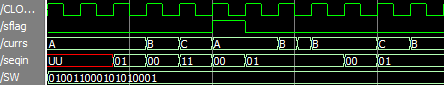
\includegraphics[width=0.8\textwidth,height=4cm,keepaspectratio]{simulation.png}
    \caption{FSM Simulation Results}
    \label{fig:test_fsm}
\end{figure}

\section{\scshape Conclusions} % (fold)
\label{sec:conclusions}

There are minor changes that could be done to the lab that would increase its power consuption and modularity for use by other projects.  For example, the clock signal could be AND gated with a run signal that would allow complete removal of the clock signal to the logical subsystems.  This would allow for cleaner code inside the PISO module that would in turn make error checking in the FSM much easier.

Overall, this lab goes to show that there two very similar, yet distinct ways to design and model finite state machines.  By using a Mealy model, this lab is able to show that even though there may be inherant risk for data instability, that risk is either minute enough to ignore or can be controlled by outside systems.  This lab also clearly demonstrates the power and versatiliy of FSM logic.

% section scshape_conclusions (end)

% Bibliography

\clearpage

\bibliography{citationsfile}{}

\clearpage

\chapter*{\scshape Appendix A: Lab 2 System}
\label{app:a}

\vspace{15px}
\begin{lstlisting}
library ieee,work;
use ieee.std_logic_1164.all;
use work.all;

entity Lab2 is
  port (
    KEY      : in  std_logic_vector(1 downto 0);
    CLOCK_50 : in  std_logic;
    SW       : in  std_logic_vector(17 downto 0);
    LEDR     : out std_logic_vector( 2 downto 0) := "000"
  );
end entity Lab2;

architecture behav of Lab2 is
  -- Thaipsch
  type state is (A,B,C,D);

  -- Schignuls
  signal currs : state;
  signal sflag : std_logic := '0';
  signal seqin : std_logic_vector(1 downto 0);
  signal count : integer range 0 to 3;

  -- Pair-El-El to Cereal Owt-Puht
  component PISO is
    port (
      clk,load : in  std_logic;
      pin      : in  std_logic_vector(17 downto 0);
      sout     : out std_logic_vector( 1 downto 0)
    );
  end component PISO;

  -- Kowntur
  component counter is
    port (
      reset  : in  std_logic;
      flag   : in  std_logic;
      clock  : in  std_logic;
      cntout : out integer range 0 to 3
    );
  end component counter;    

  -- Ark-It-Eck-Sure
begin
  -- Peeso Kumpownent
  peeso : PISO PORT MAP (
    clk              => CLOCK_50,
    load             => KEY(1),
    pin(17 downto 0) => SW(17 downto 0),
    sout             => seqin
  );

  -- Kowntur Kumpownent
  kowntur : counter PORT MAP (
    reset            => KEY(0),
    flag             => sflag,
    clock            => CLOCK_50,
    cntout           => count
  );

  -- Ef-Esh-Ehm Lawjick
  fsm_lawjick : process (CLOCK_50, seqin, KEY(0))
  begin
    if (KEY(0) = '0') then
      currs <= A;
      sflag <= '0';
    elsif (rising_edge(CLOCK_50)) then
      sflag <= '0';
      case currs is
        when A =>
          if (seqin = "01") then currs <= B; end if;
        when B =>
          if (seqin = "00") then currs <= C;
          elsif (seqin = "11") then currs <= D;
          elsif (seqin = "01") then currs <= B;
          else currs <= A; end if;
        when C =>
          if (seqin = "00" or seqin = "11") then
            sflag <= '1';
            currs <= A;
          elsif (seqin = "01") then currs <= B;
          else currs <= A; end if;
        when D =>
          if (seqin  = "00") then
            sflag <= '1';
            currs <= A;
          elsif (seqin = "01") then currs <= B;
          else currs <= A; end if;
        when others =>
          currs <= A;
      end case;
    end if;
  end process fsm_lawjick;

  -- Ellie-Dee Lawjick
  elliedee : process (count)
  begin
    case count is
      when 1 =>
        LEDR(2) <= '0';
        LEDR(1) <= '0';
        LEDR(0) <= '1';
      when 2 =>
        LEDR(2) <= '0';
        LEDR(1) <= '1';
        LEDR(0) <= '1';
      when 3 =>
        LEDR(2) <= '1';
        LEDR(1) <= '1';
        LEDR(0) <= '1';
      when others =>
        LEDR(2) <= '0';
        LEDR(1) <= '0';
        LEDR(0) <= '0';
    end case;
  end process elliedee;

end architecture behav;
\end{lstlisting}

\chapter*{\scshape Appendix B: FSM Testbench}
\label{app:b}

\vspace{15px}
\begin{lstlisting}
library ieee,work;
use ieee.std_logic_1164.all;
use work.clk_package.all;
use work.all;

entity test2 is --test-bench
end entity test2;

architecture behav of test2 is
  component lab2 is
    port (
      KEY      : in  std_logic_vector(1 downto 0);
      CLOCK_50 : in  std_logic;
      SW       : in  std_logic_vector(17 downto 0);
      LEDR     : out std_logic_vector( 2 downto 0)
    );
  end component;

  signal keyt   : std_logic_vector( 1 downto 0) := "00";
  signal clockt : std_logic;
  signal swst   : std_logic_vector(17 downto 0);
  signal ledrt  : std_logic_vector( 2 downto 0);

  signal run    : std_logic := '1';

begin

  labtest : lab2
  port map (keyt, clockt, swst, ledrt);

  clk_gen(clockt, 50.000E6, 0 fs, run);

  test : process is
  begin
    swst  <= "010011000101010001";
    keyt(0) <= '1'; wait for 25 ns;
    keyt(1) <= '1'; wait for 127 ns;
    keyt(0) <= '0'; wait for 3 ns;
    keyt(0) <= '1'; wait;

  end process;

end architecture behav;
\end{lstlisting}

\chapter*{\scshape Appendix C: PISO Testbench}
\label{app:b}

\vspace{15px}
\begin{lstlisting}
library ieee,work;
use ieee.std_logic_1164.all;
use work.clk_package.all;
use work.all;

entity testpiso is --test-bench
end entity testpiso;

architecture behav of testpiso is
  -- Pair-El-El to Cereal Owt-Puht
  component PISO is
    port (
      clk,load : in  std_logic;
      pin      : in  std_logic_vector(17 downto 0);
      sout     : out std_logic_vector( 1 downto 0)
    );
  end component PISO;

  signal clockt : std_logic;
  signal load   : std_logic;
  signal swst   : std_logic_vector(17 downto 0);
  signal outdt  : std_logic_vector( 1 downto 0);

  signal run    : std_logic := '1';

begin

  pisotest : piso
  port map (clockt,load,swst,outdt);

  clk_gen(clockt, 50.000E6, 0 fs, run);

  test : process is
  begin
    swst  <= "010011000101010001";
    load <= '1'; wait for 1 ns;
    load <= '0'; wait for 10 ns;
    load <= '1'; wait;

  end process;

end architecture behav;
\end{lstlisting}

\chapter*{\scshape Appendix D: Counter Testbench}
\label{app:b}

\vspace{15px}
\begin{lstlisting}
library ieee,work;
use ieee.std_logic_1164.all;
use work.clk_package.all;
use work.all;

% entity testcounter is --test-bench
end entity testcounter;

architecture behav of testcounter is
  -- Kowntur
  component counter is
    port (
      reset  : in  std_logic;
      flag   : in  std_logic;
      clock  : in  std_logic;
      cntout : out integer range 0 to 3
    );
  end component counter;

  signal clock  : std_logic;
  signal reset  : std_logic := '1';
  signal flag   : std_logic := '0';
  signal cntout : integer range 0 to 3;

  signal run    : std_logic := '1';

begin

  countertest : counter
  port map (reset,flag,clock,cntout);

  clk_gen(clock, 50.000E6, 0 fs, run);

  test : process is
  begin
    wait for 20 ns;
    flag  <= '1'; wait for 5 ns;
    flag  <= '0'; wait for 15 ns;
    flag  <= '1'; wait for 5 ns;
    flag  <= '0'; wait for 15 ns;
    flag  <= '1'; wait for 5 ns;
    flag  <= '0'; wait for 10 ns;
    reset <= '0'; wait for 1 ns;
    reset <= '1'; wait for 24 ns;
    flag  <= '1'; wait for 5 ns;
    flag  <= '0'; wait for 15 ns;
    flag  <= '1'; wait for 5 ns;
    flag  <= '0'; wait;

  end process;

end architecture behav;
\end{lstlisting}

%% END EDITS HERE %%

\end{spacing}

\end{document}

%%%%%%%%%%%% Extra stuff for use later

% \begin{itemize}[noitemsep,nolistsep]
%     \item \emph{Choose off-the-shelf parts} rather than self-made parts whenever possible.
%     \item \emph{Reuse and expand on open-source software libraries} to avoid spending time writing code that duplicates functionality that already exists elsewhere (and is likely more robust).
%     \item \emph{Keep the hardware simple} by using the least amount of hardware necessary for operation to avoid additional potential points of failure.
%     \item \emph{Modularize systems and components}. Each component should do one thing and do it well.
% \end{itemize}
% Figure \ref{BlockDiagram} shows a block diagram of the subsystems used in our design.

% \begin{figure}[H]
%     \centering
%     \caption{Block Diagram of Subsystems}
%     \label{BlockDiagram}
% \end{figure}
%     {
%     \centering
%       \includegraphics[width=\textwidth]{CostAccounting}
%     }